\section{Problema 2: Horizontes lejanos}

\subsection{Presentaci\'on del problema}
%aca ponemos una interpretacion de lo que nos pide el enunciado y algunas aclaraciones de como vamos a encarar el problema.
Dado un conjunto de rectángulos en un plano, todos apoyados sobre una linea recta horizontal, como en las siguientes figuras, se pide eliminar las líneas que colisionen con algún otro rectángulo, donde colisionar también es sólamente ``tocar'' otra línea.
\begin{figure}[ht]
	\begin{minipage}[t]{0.5\linewidth}
		\centering
		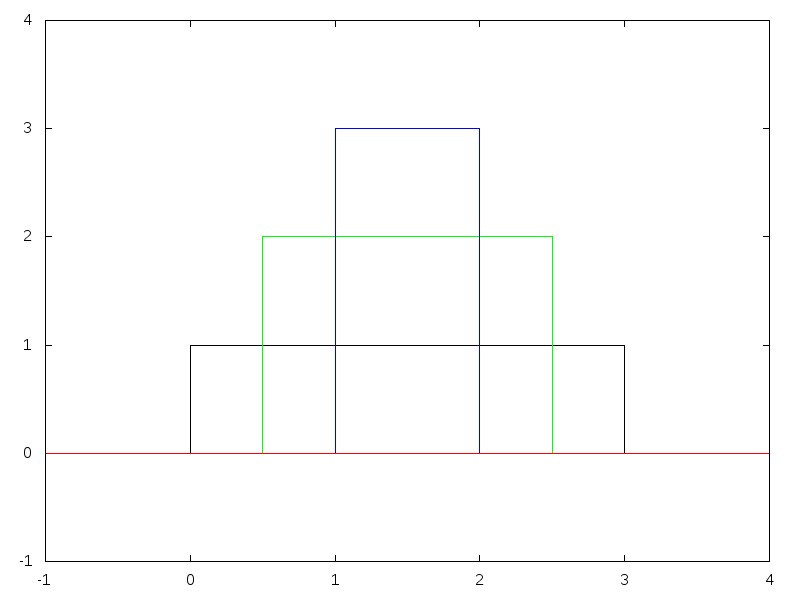
\includegraphics[width=\textwidth]{p1_ej1_pre.jpg}
		\caption{Con colisión total}
		\label{fig:p1_ej1_pre}
	\end{minipage}
	\begin{minipage}[t]{0.5\linewidth}
		\centering
		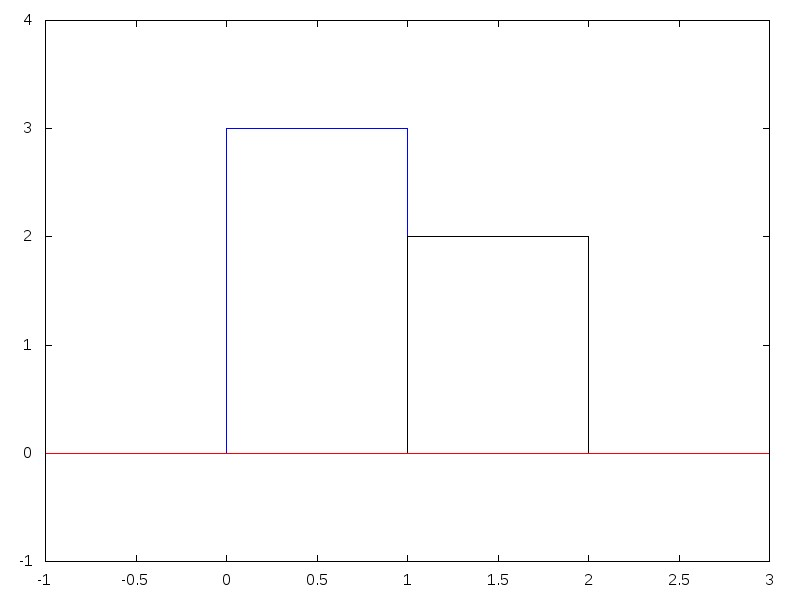
\includegraphics[width=\textwidth]{p1_ej2_pre.jpg}
		\caption{Sólo se tocan los bordes}
		\label{fig:p1_ej2_pre}
	\end{minipage}
\end{figure}

\noindent Así, tras ejecutar el algoritmo, el resultado para los ejemplos anteriores sería:

\begin{figure}[ht]
	\begin{minipage}[t]{0.5\linewidth}
		\centering
		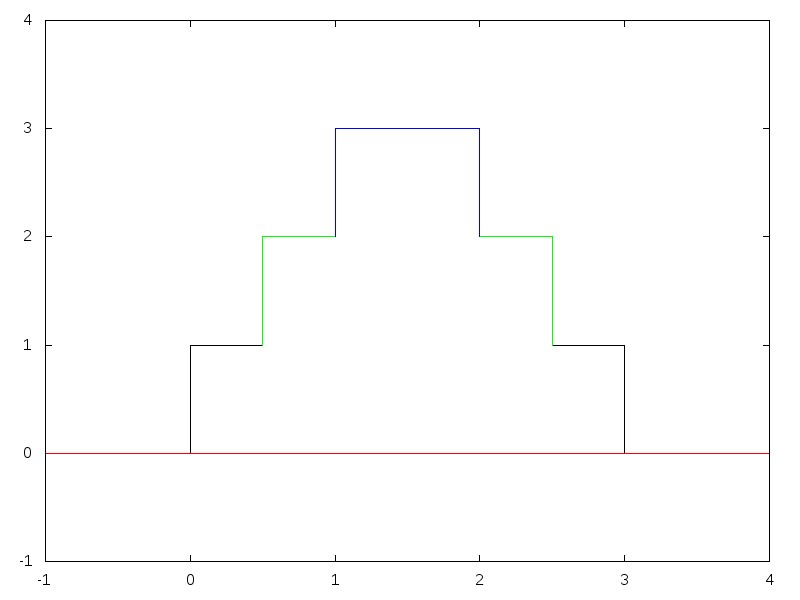
\includegraphics[width=\textwidth]{p1_ej1_post.jpg}
		\caption{Resultado con colisión total}
		\label{fig:p1_ej1_post}
	\end{minipage}
	\begin{minipage}[t]{0.5\linewidth}
		\centering
		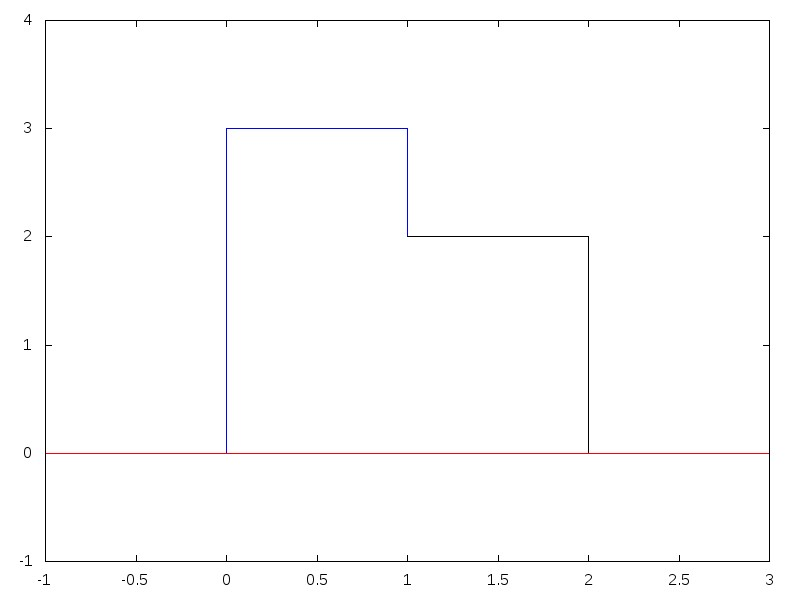
\includegraphics[width=\textwidth]{p1_ej2_post.jpg}
		\caption{Resultado cuando sólo se tocan los bordes}
		\label{fig:p1_ej2_post}
	\end{minipage}
\end{figure}

Como requerimiento adicional, el algoritmo para $n$ rectángulos debe tener una complejidad temporal estrictamente menor que $O(n^2)$.

\subsection{Resoluci\'on}
\subsubsection{Algoritmo}
Como introducción al pseudocódigo de nuestra implementación describiremos las ideas que lo respaldan para facilitar 
la asimilación del mismo. El algoritmo es muy simple pero tiene un par de puntos sutiles sobre los
que vale la pena hacer hincapié. A grandes rasgos se basa en los siguientes puntos:
\begin{enumerate}
	\item divide a los edificios en eventos de apertura y cierre
	\item ordena los eventos convenientemente
	\item itera el conjunto de eventos y va a agregando a su solución parcial los puntos en los que
	identifica cambios de altura (forma en la que definimos los puntos del contorno)
\end{enumerate} 
Cada edificio se representa con un evento de apertura y uno de cierre. Los dos eventos van a compartir la altura
original del edificio pero van a diferir en la coordenada $x$ que van a llevar: uno se quedará con la correspondiente
al inicio del edificio y el otro con la correspondiente a la finalización del mismo. 
El orden es más fácil pensarlo como una suerte de Radix Sort. Primero se ordena los eventos por su coordenada
$x$. Luego entre, entre los que comparten su coordenada $x$, se deja primero a los eventos de apertura y luego
a los de cierre. Finalmente, entre los que comparten coordenada $x$ y tipo, se ordena: en orden decreciente de altura
a los de tipo apertura y en orden creciente a los de tipo cierre. Vamos a mostrar la conveniencia de este orden
mostrando casos en los que traería problemas si estuvieran desordenados con respecto al criterio que recién describimos:
\begin{itemize}
	\item desordenados con respecto a $x$: tenemos dos edificios $e^1$ y $e^2$ superpuestos de forma tal que
	$e^1_p < e^2_p < e^1_f < e^2_f$ y $e^1_h > e^2_h$. Si iteramos primero $e^2$ vamos a suponer que en el comienzo
	del mismo hay un punto del contorno porque $e^1$ todavía no sabemos que estaba abierto.
	\item mismo $x$, desordenados respecto al tipo: suponemos que los eventos están todos correctamente ordenados
	con respecto a su coordenada $x$, sin embargo, dentro de los que comparten una misma coordenada $x$ a veces primero
	se colocó a los de cierre y luego a los de apertura. El problema que puede traer esto es que cuando yo veo
	un evento de cierre que era el que daba la altura máxima al contorno para obtener la nueva altura del contorno
	me fijo en los edificios que está abiertos. Si no cuento en ese momento con todos los que están abiertos
	en ese $x$ entonces puede que registre que el punto del contorno es diferente de lo que debería haber sido
	de saber que los que todavía no iteré de apertura estaban abiertos.
	\item eventos de apertura en orden creciente: supongamos que sólo tenemos 3 edificios, los 3 empiezan en
	la misma coordenada $x$ y los itero en orden creciente de altura. Cada vez que itero por uno de los eventos 
	de apertura me va a decir que la nueva altura es mayor a la que ya tengo del contorno por lo cual va a
	ingresar un nuevo punto al contorno, resultando en 3 puntos del contorno con el mismo $x$.
	\item eventos de cierre en orden decreciente: es muy similar al anterior, necesito haber cerrado los más
	bajos primero porque si no cuando cierro el más alto pienso que los que se van a cerrar en esa misma
	coordenada $x$ todavía están abiertos cuando en realidad no están abiertos en esa coordenada $x$, simplemente
	como los eventos se computan de a uno el orden es muy importante.
\end{itemize}
Además, queremos aclarar que para saber en todo momento qué edificios están abiertos mantenemos actualizada
una estructura con ésta información. La estructura no contiene los edificios que están abiertos, contiene
las alturas de los edificios que están abiertos. Con esta información basta ya que en todo momento
a nosotros nos interesa saber qué alturas tenemos disponibles para nuestro contorno, independientemente
del edificio al que pertenezcan. Cuando iteramos sobre un evento de apertura agregamos su altura a la 
estructura, cuando iteramos sobre un evento de cierre eliminamos un elemento con valor igual a la altura
del mismo.

\subsubsection{Pseudoc\'odigo}
%aca va el pseudocodigo del problema.
\begin{algorithm}[H]
\begin{algorithmic}
\STATE $eventos$ $\gets$ extraer\_eventos($edificios$)
\STATE $contorno_{parcial}$ $\gets$ $secuencia\_vacia$
\STATE $h_{actual}$ $\gets$ 0
\WHILE {$eventos$ $\neq$ $\emptyset$}
	\STATE $ev$ $\gets$ proximo\_evento($eventos$)
	\IF {abre($ev$)}
		\IF {$h_{actual}$ $<$ $ev_h$}
			\STATE $h_{actual}$ $\gets$ $ev_h$
			\STATE AgregarAtrás($<ev_x, ev_h>$, $contorno_{parcial}$)
		\ENDIF
	\ELSE
		\IF {$h_{actual}$ = $ev_h$ $\land$ maxAbierto($ev_x$) $<$ $h_{actual}$}
			\STATE $h_{actual}$ = maxAbierto($ev_x$)
			\STATE AgregarAtrás($<ev_x, h_{actual}>$, $contorno_{parcial}$)  
		\ENDIF
	\ENDIF
\ENDWHILE
\caption{horizontes\_lejanos}
\end{algorithmic}
\end{algorithm}

\begin{algorithm}[H]
\begin{algorithmic}
	\STATE $min_x$ = min( $\{ ev_x | ev \in eventos\}$ )
	\STATE $comparten\_min_x$ = $\{ ev \in eventos | ev_x = min_x \}$
	\IF {quedanEventosDeApertura($comparten\_min_x$)}
		\STATE $comparten\_min_x$ = filtrarLosDeCierre($comparten\_min_x$)
		\RETURN mayorAltura($comparten\_min_x$)
	\ELSE
		\RETURN menorAltura($comparten\_min_x$)
	\ENDIF
\caption{proximo\_evento}
\end{algorithmic}
\end{algorithm}

\subsection{Demostraci\'on}
\paragraph{Edificio}
Definiremos un edificio $e$ como una tupla $<e_{principio}$, $e_{final}$, $e_{altura}>$, la escribiremos de la siguiente forma por ser más compacta $<e_p$, $e_f$, $e_h>$, que cumple la siguiente propiedad:
\begin{displaymath}
	e_p, e_f, e_h \in \mathbb{N} \land e_p > 0 \land e_p < e_f \land e_h > 0
\end{displaymath}
La misma representa a un edificio $e$ que empieza en $e_p$, tiene una altura de $e_h$ y termina en $e_f$. 
Representados bidimensionalmente sobre un eje cartesiano los valores $e_p$ y $e_f$ se corresponden con
sus coordenadas sobre el eje de las abscisas $X$.

\paragraph{Evento}
Definiremos un evento como una tupla $<ev_x$, $ev_h$, $ev_t>$ que cumple la siguiente propiedad:
\begin{displaymath}
	ev_x, ev_h, ev_t \in \mathbb{N} \land ev_t \in \{ 1, 0\}
\end{displaymath}
$ev_x$ representa el valor de la coordenada $x$ del evento, $ev_h$ la altura del evento y $ev_t$ el tipo de 
evento, 1 para un evento que representa el comienzo de un edificio y 0 para los eventos que representan el fin de un edificio.
Dado un edificio $e = <e_p$, $e_f$, $e_h>$  diremos que dos eventos lo representan $ev_{abrir} = <e_p$, $e_h$, $1>$ y $ev_{cerrar} = <e_f$, $e_h$, $0>$.
Es decir, que cada edificio lo representamos con dos eventos, uno que marca el comienzo y otro que marca el fin del mismo. 
Dado un conjunto $E$ de edificios decimos que el conjunto $Ev$ de eventos que lo representa es aquel que contiene dos eventos
por cada edificio de $E$ derivados de la forma antes mostrada.

\paragraph{Contorno}
Dado un conjunto de edificios $E$ definiremos una función $h$ que toma un $x \in \mathbb{N}$ y un conjunto de edificios:
\begin{displaymath}
	h: (x,E) \to \mathbb{N} 
\end{displaymath}
$h$ nos devuelve la altura del edificio más alto que cubre ese valor de $x$ 
\begin{displaymath}
	h(x, E) = \begin{cases} 
						0 & \nexists e \in E | (x \geq e_p \land x < e_f) \\
						max\{ e_h | e \in E  \land e_p \leq x \land x < e_f \} & \exists e \in E | (x \geq e_p \land x < e_f)
				\end{cases} %\pmod{2}
\end{displaymath}
contando con $h$ ya podemos definir correctamente nuestro conjunto de puntos que conforman el contorno del
conjunto de edificios $E$:
\begin{displaymath}
	C = \{ p \in \mathbb{N}^2 | h(p_x - 1, E) \neq h(p_x, E) \land (\exists ev \in Ev | ev_x = p_x \land ev_h = p_y) \}
\end{displaymath}
Es decir, los puntos que pertenezcan al conjunto $contorno$ registrarán los cambios de altura. Cada punto
del contorno puede interpretarse como: a partir de este $p_x^i$ y hasta el $p_x^{i+1}$ el edificio con mayor
altura en todo el rango tiene altura igual a $p_y^i$ (asumiendo que los $p^i$ del contorno están ordenados
de forma creciente por su coordenada $x$). Los cambios de altura pueden producirse
porque un edificio empiece o porque un edificio haya concluido. 
Dado un conjunto de edificios $E$ existe un único conjunto $C$ que representa su contorno. 
Vale la pena aclarar que por como está planteado el problema la función $h$ nos dice que si tenemos un conjunto $E$
de edificios que sólo contiene un edificio $e = <e_p, e_f, e_h>$ entonces $h(e_p, E) = e_h$ pero $h(e_f, E) = 0$.
La altura de los edificio representa de esta forma un intervalo cerrado a izquierda pero abierto a derecha
respecto a la información que el contorno registra.

\textbf{Correctitud}
\par
A continuación se presenta el pseudocódigo de nuestra implementación sobre el cual plantearemos la
demostración de correctitud:

De ahora en más vamos a referirnos como $contorno$ a la secuencia que contiene a todos los elementos de
el conjunto de contorno $C$ ordenados por su coordenada $p_x^i$. Además, vamos a referirnos a que un
edificio $e$ contiene o abarca a un valor $x$ cuando $x \in [e_p, e_f)$.

Vamos a demostrar algunos lemas que nos servirán para realizar la demostración.

\paragraph{Lema 1}
Todos los puntos pertenecientes a $C$ satisfacen:
\begin{enumerate}
	\item $(\forall p \in C) \exists ev \in Eventos \text{ / } p_x = ev_x$
\end{enumerate}
La propiedad se desprende de la misma definición del conjunto $contorno$. Como $h(p_x, Edificios) \neq h(p_x - 1, Edificios)$ 
necesariamente ese cambio en la función de altura tiene que haberse producido porque un edificio 
$e = <e_p$, $p_x$, $h(p_x-1, Edificios)>$ concluyó, en el caso de que $h(p_x, Edificios) < h(p_x - 1, Edificios)$, o porque un
edificio $e = <p_x$, $e_f$, $h(p_x, Edificios)>$ comenzó, en el caso de que $h(p_x, Edificios) > h(p_x - 1, Edificios)$, ya que 
la altura por defecto para cualquier valor de $x$ que no esté contenido por un edificio del conjunto de edificios es 0. En los dos
casos tenemos un edificio que empieza o termina en $p_x$. Como el conjunto $Eventos$ contiene precisamente un evento por cada comienzo
y fin de un edificio, en particular contiene a los que satisfacen en cada caso la propiedad expresada.

\paragraph{Lema 2}
Sea S la secuencia de eventos tal que:
\begin{displaymath}
	ev \in S \Leftrightarrow ev \in Eventos
\end{displaymath}
de forma tal que el orden en el que se encuentran es el impuesto por agregarlos en el orden en el que la función 
proximo\_evento($Eventos$) los devuelve. Se cumple que:
\begin{displaymath}
	(\forall ev^1, ev^2 \in Eventos \text{ / } ev^1_x = ev^2_x) ev^1_h * ev^1_t > ev^2_h * ev^2_t \Rightarrow posicion(ev^1, S) < posicion(ev^2, S)
\end{displaymath}
Los casos que podemos tener son los siguientes:
\begin{enumerate}
	\item $\text{abre}(ev^1) \land \neg\text{abre}(ev^2)$  en este caso vemos que necesariamente $ev^1$ va a ser devuelto
	primero por proximo\_evento() porque siempre si los eventos comparten la coordenada $x$ prioriza los de apertura
	con la función filtrarLosDeCierre(Eventos).
	\item $\text{abre}(ev^1) \land \text{abre}(ev^2)$  podemos ver en el algoritmo de proximo\_evento() que cuando luego
	de filtrar por $min_x$ y quedarse con los de apertura en caso de que existan, estamos en el caso de que existen,
	$ev_1$ y $ev_2$ cumplen, devuelve primero el de mayor altura. Con lo cual la posición del de mayor altura
	necesariamente es menor.
\end{enumerate}
$\square$

\paragraph{Lema 3}
Sea $contorno$ la secuencia de puntos del contorno $C$ ordenados por su coordenada $x$. La secuencia tiene 
$n+1$ puntos $p^0,...,p^n$:
\begin{displaymath}
	(\forall x \in \mathbb{N} \text{ / } x < p_x^0 \lor x \geq p_x^n) h(x, E) = 0
\end{displaymath}
y además:
\begin{displaymath}
	(\forall x \in \mathbb{N} \text{ / } x \geq p_x^0 \land x < p_x^n) h(x, E) = p_y^{maxXmenor}
\end{displaymath}
con $p_y^{maxXmenor}$ igual al $p_y$ del $p$ que tiene el máximo $p_x$  de todos los $p$ que cumplen $p_x \leq x$.

La primer propiedad predica que antes del primer edificio y después del último, asumiendo un orden por coordenada $x$,
la función $h$ siempre vale 0. Estose desprende directamente de su definición, si todavía no empieza ningún edificio o
si ya terminaron todos es imposible que la altura valga algo mayor a 0 porque por defecto vale 0.
La segunda propiedad nos dice que entre dos puntos $p^1$, $p^2$ consecutivos del contorno la función $h$ necesariamente tiene
que devolvernos $p_y^1$. Si no fuera así entonces existiría un $x$ entre $p_x^1$ y $p_x^2$ en el cual $h(x, Edificios)$ nos devuelve
distinto de $p_y^1$. Como $p_y^1 = h(p^1_x, Edificios)$, por definición de contorno debería existir un punto $p$ del mismo
tal que $p_x = x$. Pero $x$ se encuentra entre $p_x^1$ y $p_x^2$ que son puntos consecutivos del contorno por lo cual no
puede existir ningún cambio de altura entre ellos ya que si existiera debería haber un punto del contorno allí y eso es
absurdo porque presumimos que eran consecutivos.
$\square$
 
Nuestro algoritmo consiste en un ciclo que itera sobre todos los elementos de $Eventos$. Vamos a demostrar
que el ciclo cumple el siguiente invariante:
\begin{displaymath}
	esPrefijo(contorno_parcial, contorno) 
\end{displaymath}

\textbf{Antes de entrar al ciclo}
\par
Antes de entrar al ciclo $contorno_{parcial} = secuencia\_vacia$. La secuencia vacía es prefijo de todas las secuencias, por lo tanto
el invariante se cumple antes de entrar al ciclo por primera vez.
\par
\textbf{El ciclo preserva el invariante}
\par
Si el ciclo no agrega puntos a $contorno_parcial$ entonces necesariamente sigue siendo prefijo de $contorno$ por lo cual
el invariante se preserva. Necesitamos demostrar que lo preserva cuando agrega elementos al mismo. Llamamos $p^i$ al último 
elemento de la secuencia $contorno_{parcial}$ y $h_{actual}$ a $p^i_y$. Existen dos casos en los que agrega elementos a 
$contorno_parcial$, estos son cuando se cumplen alguna de estas dos proposiciones:
\begin{description}
	\item[Caso 1] $\text{abre}(ev) \land h_{actual} < ev_h$
	\item[Caso 2] $\neg\text{abre}(ev) \land ev_h = h_{actual} \land maxAbierto(ev_x) < h_{actual}$
\end{description}
$contorno_{parcial}$ es prefijo de $contorno$. Para que $contorno_{parcial}$ continue siendo prefijo el elemento
que agregue tiene que ser necesariamente $p^{i+1}$ en la secuencia $contorno$. $p^{i+1}_x$ es el mínimo $x$ tal que $x > p^i_x$
 y $h(x, Edificios) \neq p^i_y$. Por \textbf{Lema 1} sabemos que necesariamente existe un $ev$ tal que $ev_x = p^{i+1}_x$.
\par
Si $p^{i+1}_x > p^{i}_x$ entonces vale abre($ev$). Por \textbf{Lema 2} sabemos que nuestro algoritmo
iterará primero sobre el $ev^i$ con $ev^i_x = p^{i+1}_x \land \text{abre}(ev^i)$ de mayor altura. Entonces, necesariamente itera
primero sobre el que cumple que $ev_x = p^{i+1}_x \land h_{actual} < ev_h$. Como entra en el Caso 1 sabemos que lo va a agregar y además
sabemos que como proximo\_evento() devuelve primero los que menor coordenada $x$ tengan será el con mínimo $ev_x$ que cumple el Caso 1.
Entonces concluimos que si $p^{i+1}_x > p^{i}_x$ entonces nuestro algoritmo lo va a agregar a contorno parcial y va a ser el
primero que agregue. Por lo tanto, $contorno_{parcial}$ sigue siendo prefijo de $contorno$.
\par
El otro caso es cuando vale $p^{i+1}_x < p^{i}_x$. Ésto implica que $\neg\text{abre}(ev)$, tomando $ev$ con el que se 
corresponde con $p^{i+1}$. $ev_h = h_{actual}$ se desprende de que si fuera mayor caemos en un absurdo porque asumimos que 
$p^{i+1}_x < p^{i}_x$ y si fuera menor entonces no cambiaría la altura, lo cual lo excluiría de la definición de los 
puntos pertenecientes a $C$. Por último, es necesario que $maxAbierto(ev_x) < h_{actual}$ porque si no se cumpliera
esto no existiría tal cambio de altura, por lo cual el punto no pertenecería la contorno. Por lo tanto, el próximo punto
del contorno cae en nuestro Caso 2 y también es agregado al $contorno_{parcial}$ para que preserve la propiedad
de ser prefijo de $contorno$.
\par
Finalmente, necesitamos demostrar que la satisfacción del invariante y la negación de la guarda del ciclo implican que 
$contorno_{parcial} = contorno$. Veamos que:
\begin{enumerate}
	\item Comparten el último elemento: el último elemento de $contorno$ cumple que $p_y = 0 \land p_x = e_f^max$ con $e_f^max$
	el maximo valor de finalizacion de entre todos los edificios. Antes de $e_f^max$ $h \geq e_h^max$ y para todo $x$ mayor o igual
	a $e_x^max$ valdrá 0. Por lo tanto, es el último punto donde cambia la altura, será el último punto de mi contorno. Ese punto
	además tiene un evento correspondiente que es el último que recorre proximo\_evento() y cumple el Caso 2 por lo
	cual también será agregado.
	\item El orden que guardan sus elementos es total: esto ya lo demostramos, es simplemente que $p^i_x < p^{+1}i_x$ para 
	todos los i entre 0 y las longitud de $contorno$. 
\end{enumerate}
Estas dos propiedades y el hecho de que sea prefijo una de otra nos implica directamente que las secuencias son iguales. Por
lo tanto, al concluir el ciclo, efectivamente $contorno_{parcial} = contorno$.

\subsection{An\'alisis de complejidad}
Para calcular la complejidad del algoritmo que implementamos primero debemos
explicar cómo resolvimos en la implementación el cáculo de maxAbierto($x$) con
una estructuras de datos conveniente que nos permite realizar todas las
operaciones necesarias sin superar la cota de complejidad requerida.
Contamos con un Multiconjunto, que llamaremos $abiertos$, que nos provee la
siguiente interfaz:
\begin{itemize}
	\item inserción: $O(log n)$
	\item borrado: $O(log n)$
	\item obtención del máximo: $O(log n)$
\end{itemize}
utilizaremos esta estructura de forma tal que calcular la función maxAbierto($x$)
sea equivalente a obtener el máximo de este multiconjunto. Para ello debemos
mantenerlo actualizado, esto implica que en cada iteración si el evento es de tipo
apertura lo agregamos a $abiertos$ (costo O($log n$)). 

La complejidad de este algoritmo puede calcularse como:
\begin{displaymath}
	O(extraer_eventos) + \#eventos * O(proximo_evento) + 
\end{displaymath}


\subsection{Test de complejidad}
%aca van los graficos y todos los testeos que hagamos para probar que en la practica el algoritmo cumple la complejidad que propusimos en el punto anterior
Para \textit{testear} en la práctica la complejidad del Algoritmo, se hizo un generador de instancias de pruebas: \textit{"generadorTests.cpp"}.

Este archivo genera $10000$ instancias que son $10$ para cada valor de $n$, que es el numero de edificios que va desde $1$ hasta $1000$.
Este generador consiste en $3$ ciclos anidados, el más externo hace $n$ iteraciones, ya que se repite para cada edificio (archivo: \textit{entrada.txt} en la carpeta \textit{src/p2/}).
El segundo ciclo hace exactamente $10$ iteraciones, y es este el que hace que haya $10$ instancias para cada valor de $n$.
Por último, el ciclo más interno genera $n$ filas de tres enteros ($x, h, y$) aleatorios menores que $1000$ y con la condición de que $x$ sea menor que $y$.
Los números aleatorios son creados por la función \textit{rand()} de la librería estandard de C++.

Para probar todas estas instancias, creamos otro archivo \textit{test.cpp}, que toma entradas de este problema y devuelve las mediciones del tiempo que este tarda en correr.
Para cada instancia de prueba, éste algoritmo calcula $10$ veces el tiempo de ejecución y luego obtiene un promedio de todos los resultados. Esto minimiza posibles errores de medición y hace que los resultados sean más exactos.
Luego, promedia también los resultados para los $n$ que son iguales, obteniendo un valor de tiempo de ejecución promedio para cada valor de $n$.

Como vimos en la sección anterior, la complejidad de este algoritmo es de $O(nlog(n))$, por lo tanto, para obtener valores más graficos y más faciles de interpretar a la hora de graficar, dividimos cada resultado por $log(n)$.

Estos resultados fueron exportados a otro archivo de salida (\textit{tiempos.output}) y los resultados estan expresados a continuación:

\ponerGrafico{test2.png}{Tiempos de Ejecucion dividido log(n) de entradas aleatorias}{0.6}{}

Concluyendo a partir del gráfico de Tiempos de Ejecución, podemos afirmar que efectivamente la complejidad es $O(nlog(n))$ ya que los resultados fueron divididos por $log(n)$ y el gráfico muestra una evidente recta.

%\subsection{Testing}
%aca ponermos todos nuestros casos bordes, como actua nuestro algoritmo en los casos particulares.































